\section{Gradients request scheduling}

\subsection{Introduction}
\begin{frame}
    \frametitle{Introduction}
	\begin{itemize}
		\item Client changes gradient request order to get some benefits.  
	\end{itemize}
\end{frame}


\subsection{Some examples}
\begin{frame}
    \frametitle{Reduce suspend}
    \begin{figure}
		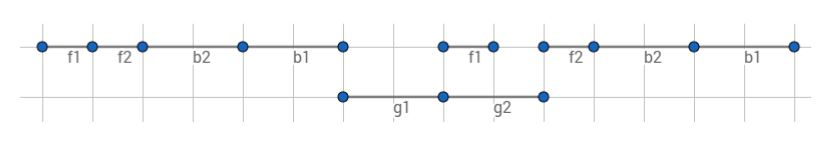
\includegraphics[scale=0.4]{figure/reducesuspend.JPG}
		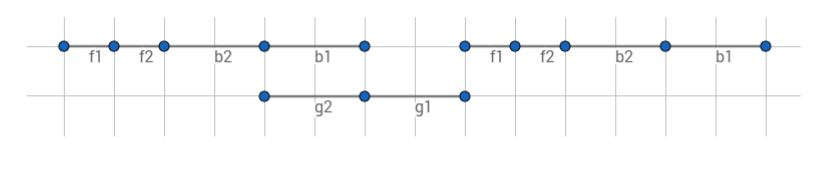
\includegraphics[scale=0.4]{figure/reducesuspend2.JPG}
	\end{figure}
\end{frame}

\begin{frame}
	\frametitle{Reduce staleness}
	\begin{figure}
		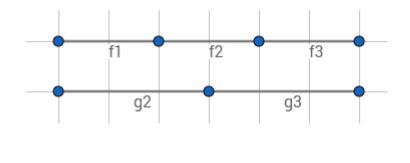
\includegraphics[scale=0.4]{figure/reducestaleness.JPG}
	\end{figure}
\end{frame}

\subsection{Problem description}
\begin{frame}
	\frametitle{Input}
	\begin{itemize}
		\item B = staleness bound.
		\item L = number of layers.
		\item I = number of iterations.
		\item W = number of workers.
		\item Cp = computation time : f1, b1, f2, b2, ...
		\item Cm = communication time : t1, t2, ...
	\end{itemize}
\end{frame}
\begin{frame}
	\frametitle{Intermediate data}
	\begin{itemize}
		\item Server maintains a set of variables indicating the minimum iteration of each layer.
		\item c1, c2, ... , cL
	\end{itemize}
\end{frame}

\begin{frame}
	\frametitle{Objective}
	\begin{itemize}
		\item Minimize training time and staleness. 
	\end{itemize}
\end{frame}

\subsection{Scheduling}
\begin{frame}
	\frametitle{Request pool}
	\begin{itemize}
		\item Pull request. 
		\item Push request. 
	\end{itemize}
\end{frame}
\begin{frame}
	\frametitle{Scheduling}
	\begin{itemize}
		\item First in first out.
		\item First in last out.
			\begin{itemize}
				\item Starvation.
			\end{itemize}
	\end{itemize}
\end{frame}
\begin{frame}
	\frametitle{Optimal solution}
	\begin{itemize}
		\item Pull
		\begin{itemize}
			\item Pull the stalest layer. 
		\end{itemize}
		\item Push
		\begin{itemize}
			\item Push the layer which can update intermediate data. 
		\end{itemize}
	\end{itemize}
\end{frame}
